
\lstset{ %
language=C,                % choose the language of the code
basicstyle=\footnotesize,       % the size of the fonts that are used for the code
numbers=left,                   % where to put the line-numbers
numberstyle=\footnotesize,      % the size of the fonts that are used for the line-numbers
stepnumber=1,                   % the step between two line-numbers. If it is 1 each line will be numbered
numbersep=5pt,                  % how far the line-numbers are from the code
backgroundcolor=\color{white},  % choose the background color. You must add \usepackage{color}
showspaces=false,               % show spaces adding particular underscores
showstringspaces=false,         % underline spaces within strings
showtabs=false,                 % show tabs within strings adding particular underscores
tabsize=2,          % sets default tabsize to 2 spaces
captionpos=b,           % sets the caption-position to bottom
breaklines=true,        % sets automatic line breaking
breakatwhitespace=false,    % sets if automatic breaks should only happen at whitespace
escapeinside={\%*}{*)}          % if you want to add a comment within your code
}

\begin{figure}[h!]
\center{
\begin{lstlisting}
pthread_t thread[MAXTHREADS];
struct thread_data data[MAXTHREADS];
void pthread_reduce(void) {
   for (i = 1; k <= nrows - 1; ++k) {
      for (i = k + 1; i <= nrows; ++i) {
         data[i] = /* Setup worker. */;
         pthread_create(&thread[i], NULL, worker,
            &data[i]);
      }

      /* Bug! Should be i <= nrows */
      for (i = k + 1; i < nrows; ++i)
         pthread_join(thread[i], NULL);
   }
}
\end{lstlisting}
\caption{pthread gaussian elimination.}}
\end{figure}

\begin{figure}[h!]
\center{
\begin{lstlisting}
/* Forks a deterministic child. Returns 0 into the
 * child and 1 into the parent. */
int dfork(pid_t childid);
/* Merges a child's changes into the parent after
 * the child issues a dret(). */
void djoin(pid_t childid);

void det_reduce(void) {
   for (i = 1; k <= nrows - 1; ++k) {
      for (i = k + 1; i <= nrows; ++i) {
         data[i] = /* Setup worker. */;
         if (!dfork(i)) { worker(&data[i]); dret(); }
      }

      /* Bug! Should be i <= nrows */
      for (i = k + 1; i < nrows; ++i)
         djoin(i);
   }
}
\end{lstlisting}
\caption{Deterministic Gaussian elimination.}}
\end{figure}

\begin{figure}[t]
\center{
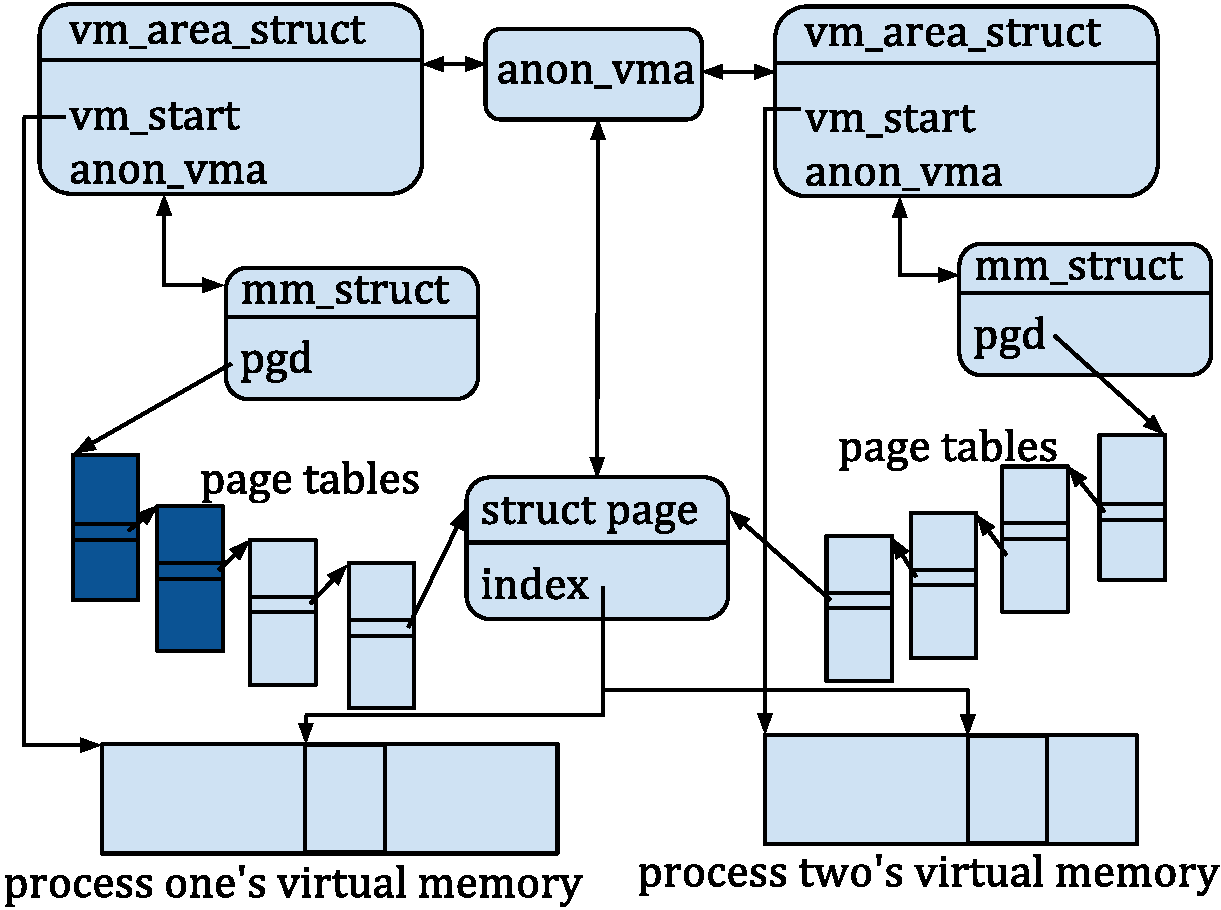
\includegraphics[scale=.35]{anon_vma_highlight.pdf}
\caption{Data structure relationships associated with object-based reverse
mapping. The {\tt struct page} C type encapsulates information about every
page frame of physical memory.
Two processes map virtual memory to the same page read-only (possibly
at different addresses). In order for the kernel to swap a given page to disk,
object-based reverse mapping assumes each process maps the page to
\mbox{{\tt vm\_area\_struct->vm\_start} + {\tt page->index}} in virtual
memory.}
\label{fig:anon_vma}}
\end{figure}

\begin{figure}[h!]
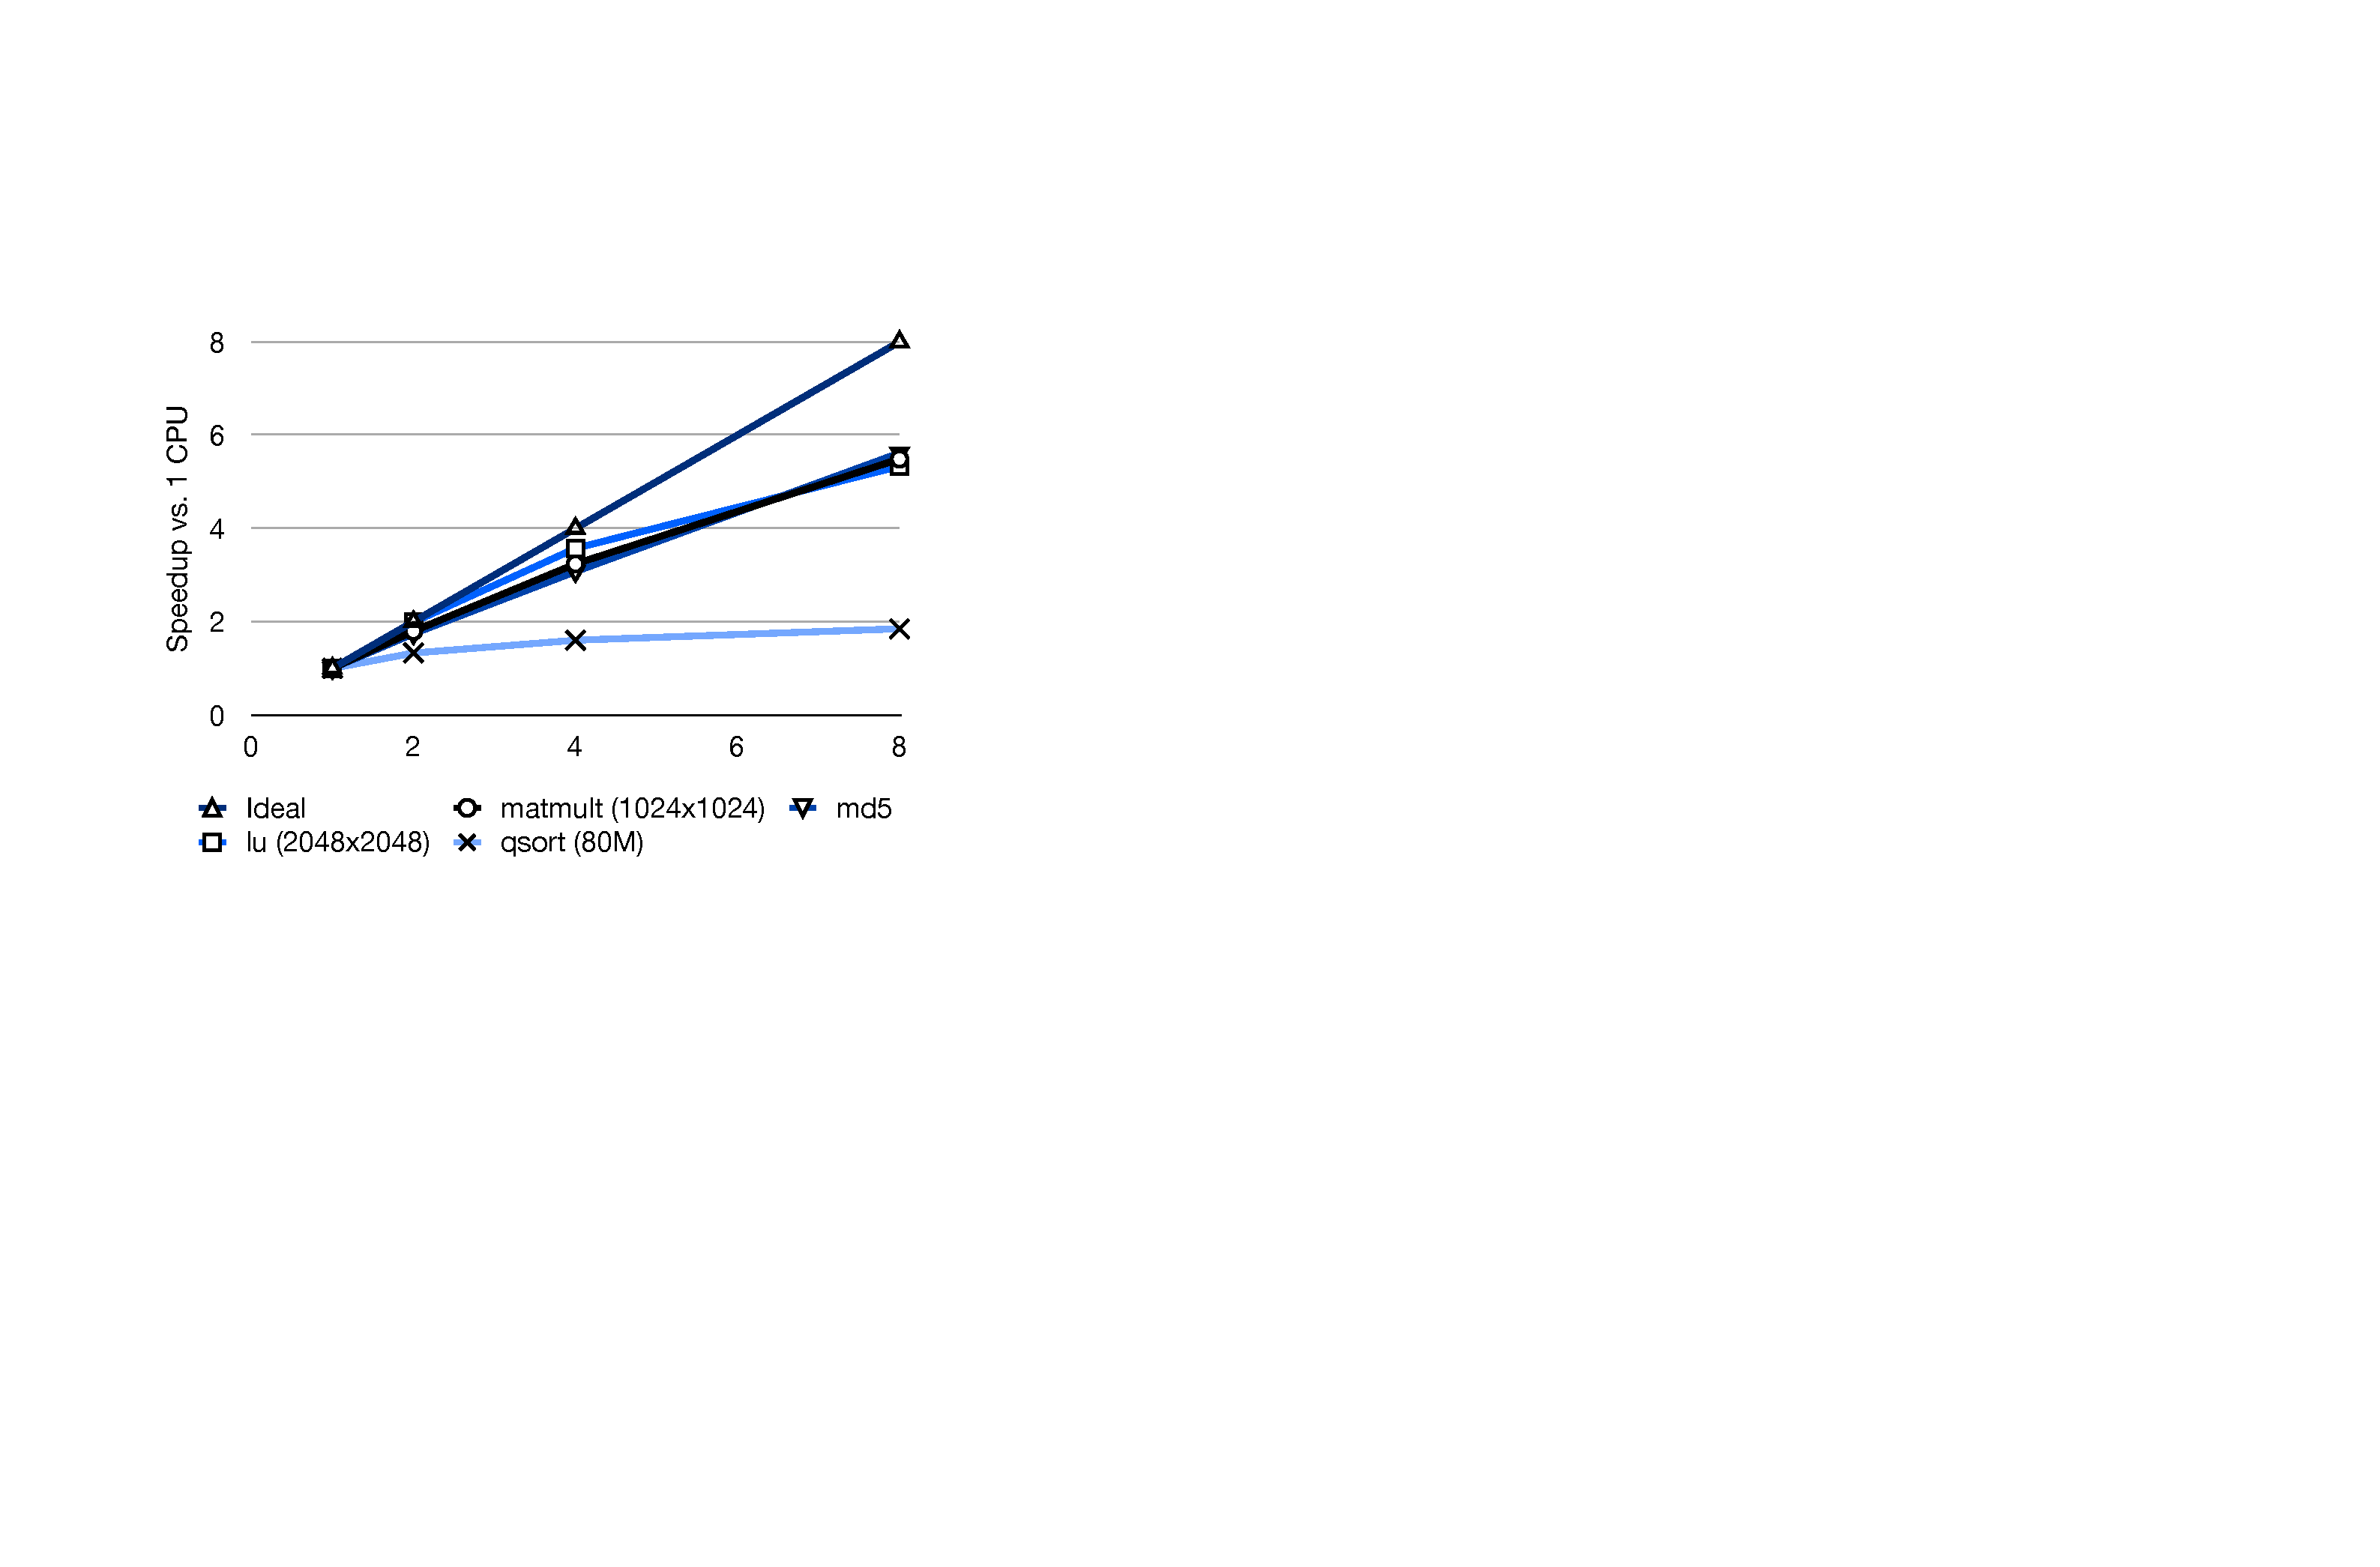
\includegraphics[scale=.57]{dspeedup.pdf}
\caption{Deterministic speedup for the parallel benchmarks.}
\label{fig:dspeedup}
\end{figure}

\begin{figure*}[h!]
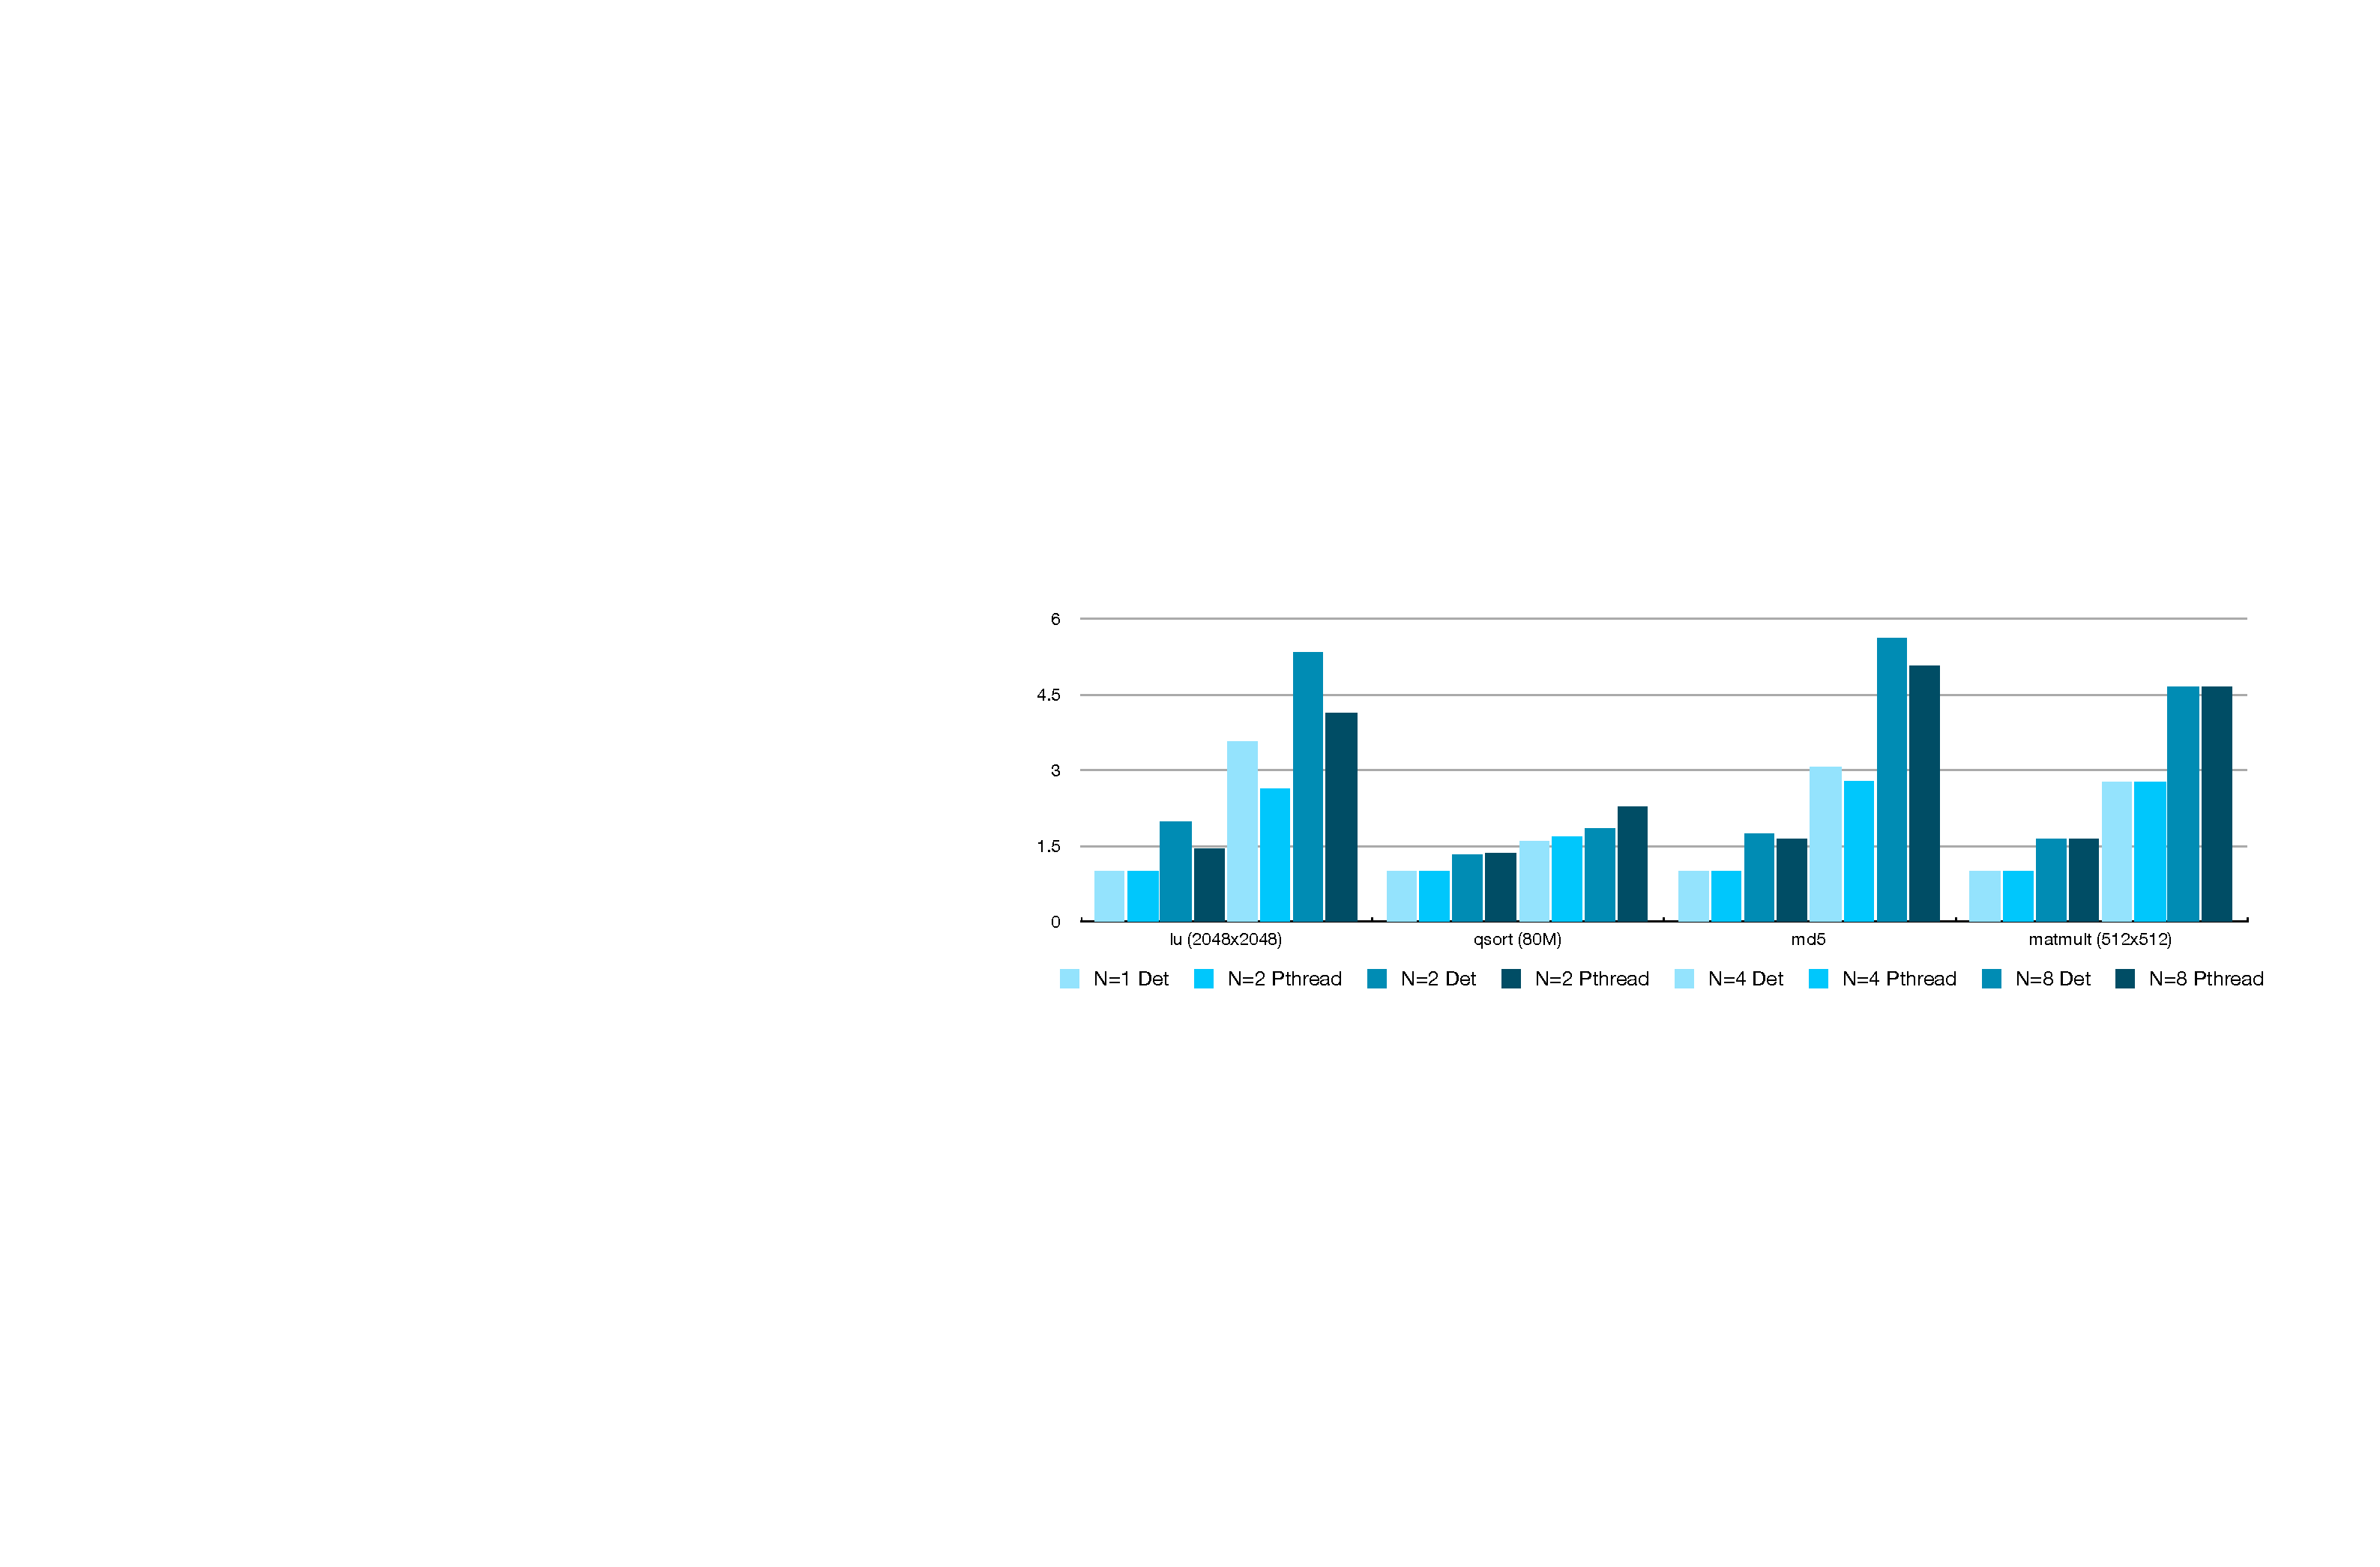
\includegraphics[scale=.7]{scale.pdf}
\caption{Comparing the speedup over $N=1$ for the deterministic and pthread
versions of the benchmarks. This figure demonstrates the ability of both
versions to scale as we add more CPU cores.}
\label{fig:scale}
\end{figure*}

\begin{table*}[h!]
\center{
\scalebox{1}{
\begin{tabular}{|l| l l l l | l l l l |}
\hline
 & \multicolumn{4}{c|}{\textbf{lu}} & \multicolumn{4}{c|}{\textbf{matmult}} \\
Dimension & $N=1$ & $N=2$ & $N=4$ & $N=8$ & $N=1$ & $N=2$ & $N=4$ & $N=8$ \\
\hline
$16\times16$ & 13.1 (41.5\%) & 45.0 (46.7\%) & 46.3 (45.8\%) & 30.9 (31.5\%) &
  9.6 (48.2\%) & 21.8 (45.0\%) & 37.8 (45.2\%) & 16.0 (26.5\%) \\
$32\times32$ & 8.5 (34.0\%) & 37.3 (45.5\%) & 45.9 (46.1\%) & 29.1 (31.1\%) &
  3.3 (37.7\%) & 13.4 (42.0\%) & 21.1 (42.2\%) & 17.5 (24.1\%) \\
$64\times64$ & 2.6 (19.5\%) & 20.6 (41.6\%) & 42.1 (44.2\%) & 32.1 (30.9\%) &
  1.3 (13.4\%) & 3.8 (26.3\%) & 7.8 (34.0\%) & 13.2 (25.8\%) \\
$128\times128$ & 1.4 (2.3\%) & 6.0 (32.8\%) & 22.4 (39.0\%) & 30.8 (31.0\%) &
  1.0 (0.3\%) & 1.9 (1.7\%) & 4.5 (13.3\%) & 6.7 (18.2\%) \\
$256\times256$ & 1.1 (0.5\%) & 2.1 (11.0\%) & 7.0 (25.9\%) & 18.8 (31.1\%) &
  1.0 (0.0\%) & 1.2 (1.0\%) & 1.8 (1.6\%) & 2.3 (5.0\%) \\
$512\times512$ & 1.0 (0.1\%) & 1.2 (1.4\%) & 2.3 (9.4\%) & 5.9 (19.4\%) & 1.0
  (0.0\%) & 1.0 (0.5\%) & 1.1 (0.9\%) & 1.5 (3.0\%) \\
$1024\times1024$ & 1.4 (0.0\%) & 1.0 (0.3\%) & 1.2 (1.5\%) & 1.9 (8.4\%) & 1.0
  (0.0\%) & 0.9 (0.0\%) & 1.0 (0.1\%) & 1.2 (0.2\%) \\
$2048\times2048$ & 1.4 (0.0\%) & 1.0 (0.0\%) & 1.0 (0.1\%) & 1.1 (1.0\%) & - & - & - & - \\
\hline
\end{tabular}
\caption{Deterministic overhead for \emph{lu} and \emph{matmult}.
Overhead is deterministic run time divided by pthread run time.
The numbers in parentheses indicate time spent
in the kernel performing a virtual memory merge as a percentage of overall
runtime.}}}
\label{tab:matover}
\end{table*}

\endinput

